\documentclass[11pt,twocolumn]{article}
\usepackage[margin=2.2cm]{geometry}
\usepackage{times}
\usepackage{amsmath,amssymb}
\usepackage{graphicx}
\usepackage{booktabs}
\usepackage{hyperref}
\usepackage{float}
\usepackage{caption}
\usepackage{subcaption}
\usepackage{tikz}
\usetikzlibrary{positioning,arrows.meta,shapes.geometric,calc,fit,backgrounds}
\usepackage{enumitem}

\graphicspath{{../../}}

\hypersetup{colorlinks=true, urlcolor=blue, linkcolor=blue, citecolor=blue}

\title{\textbf{Deep RL for Automated Stock Trading}\\[4pt]
\large CS5242 Neural Networks and Deep Learning --- Group ID24}
\author{
Yufan Zhu \quad
Rutwik Shrikant Dharanappagoudar \quad
Xin Fei 
}
\date{Semester 2, 2025/26}

\begin{document}

\makeatletter
\twocolumn[\begin{@twocolumnfalse}
\maketitle
\begin{abstract}
\noindent
We design and implement Deep Q-Network (DQN), Double DQN (DDQN), Advantage Actor-Critic (A2C) and Proximal Policy Optimisation (PPO) in PyTorch and apply them to a single-asset stock-trading task on AAPL drawn from daily DJIA OHLCV data over 2009 to 2020. Our goal is explicitly pedagogical: to understand what each component of a deep-RL trading pipeline does when stressed by real market data. We build a Gym-style \texttt{TradingEnv} with a 10-feature technical-indicator state, a three-action position-delta action space, transaction costs and clipped log-return rewards. After diagnosing that the original RL agents underperformed passive buy-and-hold, we add a 20-day momentum feature, supervised momentum warm-starting, lower-destructive DQN exploration settings and a TDQN-inspired counterfactual replay mechanism that stores alternate-action transitions for off-policy value agents. On the 436-day out-of-sample AAPL test split spanning the COVID-19 crash of early 2020, all four RL agents now exceed buy-and-hold in cumulative return and Sharpe. PPO achieves the strongest result with $+184.3\%$ cumulative return and a Sharpe of $2.81$, while DQN and DDQN reach approximately $+172\%$ cumulative return and Sharpe above $2.72$. The exercise shows both the fragility of naive RL trading and the practical value of giving RL agents a sensible financial prior.
\end{abstract}
\vspace{1.2em}
\end{@twocolumnfalse}]
\makeatother

%====================================================================
\section{Introduction}
%====================================================================

Stock trading is naturally framed as a sequential decision-making problem in which an agent observes market state and chooses to buy, hold or sell so as to maximise long-term profit, exactly the setting targeted by Reinforcement Learning~\cite{sutton2018}. Classical rule-based trading strategies are brittle and struggle to adapt to non-stationary market dynamics, which motivates a learning-based approach.

Deep Reinforcement Learning (DRL)~\cite{mnih2015,sutton2018} learns trading policies directly from data without hand-crafted rules, and a now-substantial line of work has applied it to financial decision making~\cite{moody2001,deng2016,jiang2017,yang2020}. We implement DQN~\cite{mnih2015}, Double DQN (DDQN)~\cite{hasselt2016}, A2C~\cite{mnih2016a3c} and PPO~\cite{schulman2017ppo} in PyTorch~\cite{paszke2019} and evaluate them on historical DJIA data with AAPL as a single-asset case study. We compare against four classical baselines of increasing sophistication, namely passive buy-and-hold, an ARIMA(1,0,0) walk-forward forecaster, 20-day price momentum and a Random Forest classifier trained on the same feature set as the RL agents.

Our goal is explicitly pedagogical. We aim to understand DRL by designing and analysing these algorithms from first principles on a realistic financial task. The initial version of the project did \emph{not} beat the passive benchmark, which led us to inspect the implementation, compare against simpler trading rules and add a stronger financial prior to the RL agents. The final version therefore studies both sides of the problem: why naive RL trading is brittle, and how feature design, warm-starting and off-policy replay can materially improve performance without changing the evaluation split.

%====================================================================
\section{Data}
%====================================================================

We use the \texttt{alincijov/trading} Kaggle dataset, which provides daily OHLCV data for 30 DJIA stocks from 2009 to 2020, roughly $2{,}900$ days per ticker, downloaded programmatically via \texttt{kagglehub}. Our data pipeline loads a 10-ticker subset of the DJIA, and all experiments in this report focus on AAPL as a single-asset case study. The pipeline also supports other tickers for future multi-asset extensions. Data is split chronologically into 70\%, 15\% and 15\% train, validation and test sets, and train statistics are used for feature normalisation so as to avoid look-ahead bias.

For each ticker we compute 10 features. These are the daily return, two price deviations from short and long moving averages, 20-day trailing momentum, RSI-14, the MACD signal, Bollinger Band width, normalised volume, the Average True Range (ATR) and the On-Balance Volume (OBV). The 20-day momentum feature was added after error analysis showed that the strongest classical baseline relied on exactly this monthly trend signal, while the original state did not expose it cleanly. All features are z-score normalised using training-set statistics only to prevent data leakage. Raw returns and close prices are preserved separately for reward and portfolio computation.

\begin{figure*}[t]
  \centering
  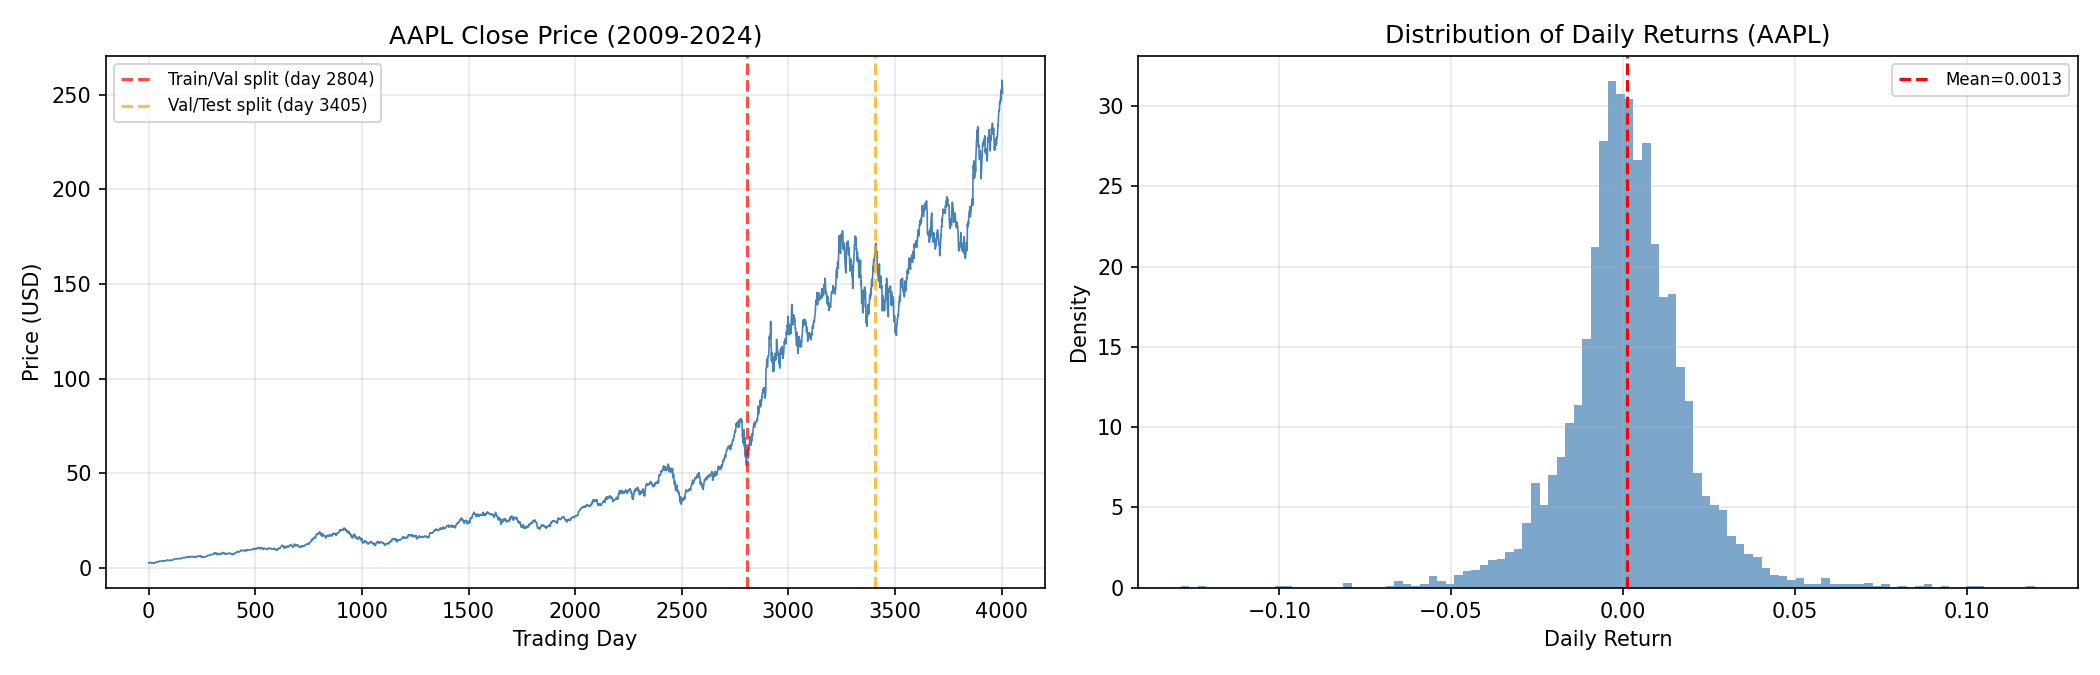
\includegraphics[width=0.95\textwidth]{results/data_exploration.png}
  \caption{\textbf{Left.} AAPL close price from 2009 to 2020 with train, validation and test boundaries. \textbf{Right.} Daily return distribution showing the characteristic fat tails of equity returns.}
  \label{fig:data}
\end{figure*}

Figure~\ref{fig:corr} shows the Pearson correlation between the engineered features on AAPL. Most pairs exhibit low correlation, which suggests limited linear redundancy among these indicators on this ticker. We treat this as a single-ticker observation rather than a general claim.

\begin{figure}[H]
  \centering
  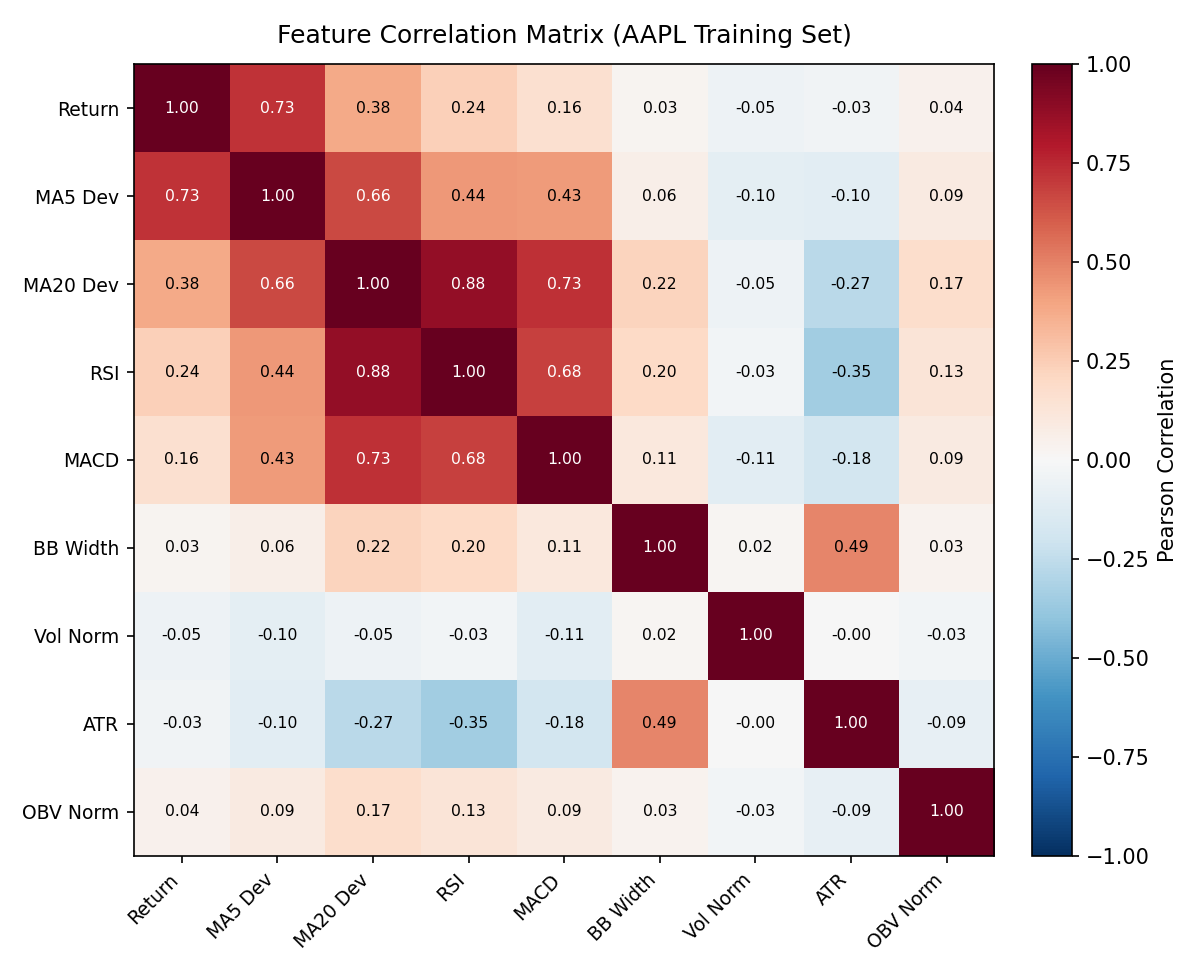
\includegraphics[width=\columnwidth]{results/feature_correlation.png}
  \caption{Feature correlation matrix on the AAPL training set. Most pairs show low linear correlation on this ticker, suggesting limited linear redundancy.}
  \label{fig:corr}
\end{figure}

The full technical indicator time series and feature distribution comparisons across splits are provided in Appendix~\ref{app:data} (Figures~\ref{fig:indicators} and~\ref{fig:distributions}).

%====================================================================
\section{Environment Design}
%====================================================================

We implement a Gym-style~\cite{brockman2016} \texttt{TradingEnv} for single-asset trading. The state $s_t \in \mathbb{R}^{11}$ concatenates the 10 normalised features with the current integer position. In the final experiments we use a long/flat trading constraint, so $\text{pos}_t \in \{0,+1\}$. The agent still chooses from three discrete position-delta actions, namely Decrease, Hold and Increase with deltas $-1$, $0$ and $+1$, but the resulting position is clamped to $[\text{pos}_{\min}, \text{pos}_{\max}] = [0,+1]$. This keeps a consistent action interface while matching the long-and-flat classical baselines used for comparison.

The reward is a clipped log-return with an explicit drawdown penalty. We first update the portfolio according to the chosen position,
\begin{equation}
  V_t = V_{t-1}\bigl(1 + \text{pos}_t \cdot \tilde r_t - c_t \cdot \mathbf{1}[\text{pos}_t \neq \text{pos}_{t-1}]\bigr),
\end{equation}
where $\tilde r_t$ is the raw un-normalised daily return and $c_t$ is a transaction cost applied only when the position changes. We then define
\begin{multline}
  r_t = \log\!\frac{V_t}{V_{t-1}} + \lambda \min\!\Bigl(0,\, \frac{V_t - V_t^{\text{peak}}}{V_t^{\text{peak}}}\Bigr),\\
  r_t \leftarrow \mathrm{clip}(r_t, -1, +1),
  \label{eq:reward}
\end{multline}
with $\lambda = 0.5$ and $V_t^{\text{peak}} = \max_{s \le t} V_s$. In all experiments $c_t$ is a flat 10~bps fee on every position change. An optional proportional mode scales the cost by $|\Delta\text{pos}|$ but is not used in this report. The log-return form is numerically stable and scale-invariant across tickers, and the drawdown term directly penalises excursions below the running portfolio peak.

Training episodes sample a random 252-day window from the 2034-day training set and therefore expose the agent to diverse market regimes per episode. Validation and test episodes always start at index~0 and run for the full split length, so the evaluation is deterministic and reproducible. The environment tracks position history, trades and portfolio value, and computes annualised Sharpe ratio, maximum drawdown and trade frequency at episode end.

%====================================================================
\section{Deep Learning Methods}
%====================================================================

Figure~\ref{fig:architecture} gives an overall view of the DQN training architecture used throughout this work. The online network $Q_\theta$ interacts with \texttt{TradingEnv} through an $\varepsilon$-greedy policy, transitions are pushed to a replay buffer, and mini-batches sampled from the buffer drive a temporal-difference loss against a slowly-updated target network $Q_{\bar\theta}$. In the final implementation, DQN and DDQN also use a TDQN-inspired counterfactual replay trick~\cite{theate2021}: after the chosen action is evaluated, the environment computes what the alternate actions would have produced from the same state and adds those synthetic off-policy transitions to replay.

\begin{figure*}[t]
\centering
\small
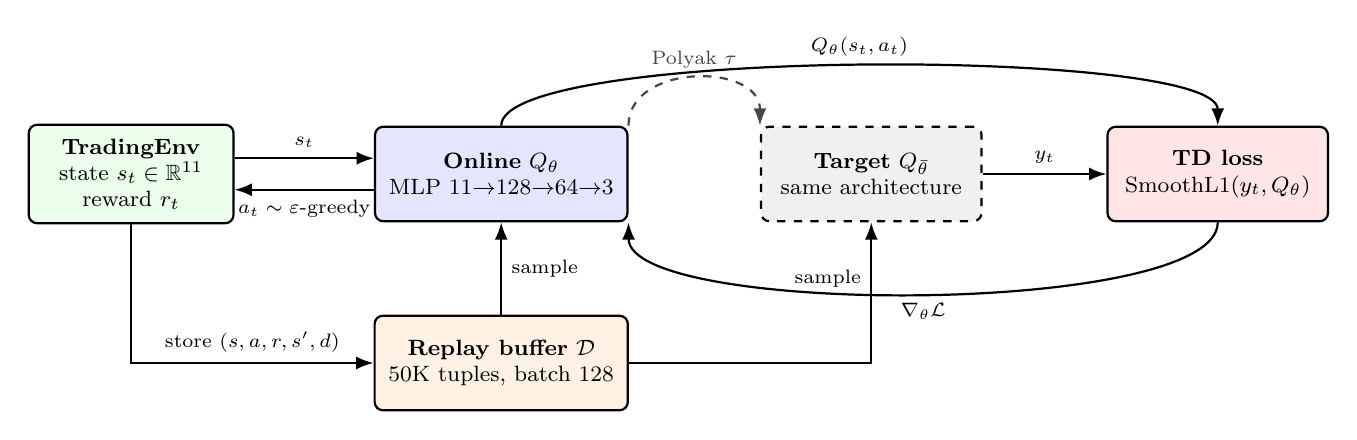
\begin{tikzpicture}[
  every node/.style={font=\footnotesize, align=center},
  env/.style  ={draw, thick, rounded corners=3pt, fill=green!8,  inner sep=5pt, minimum height=12mm, minimum width=26mm},
  net/.style  ={draw, thick, rounded corners=3pt, fill=blue!10,  inner sep=5pt, minimum height=12mm, minimum width=28mm},
  tgt/.style  ={draw, thick, rounded corners=3pt, fill=gray!12,  inner sep=5pt, minimum height=12mm, minimum width=28mm, dashed},
  buf/.style  ={draw, thick, rounded corners=3pt, fill=orange!10,inner sep=5pt, minimum height=12mm, minimum width=26mm},
  lss/.style  ={draw, thick, rounded corners=3pt, fill=red!10,   inner sep=5pt, minimum height=12mm, minimum width=28mm},
  flow/.style ={-{Latex[length=2.2mm]}, thick},
  soft/.style ={-{Latex[length=2.2mm]}, thick, dashed, gray!55!black},
]

\node[env] (env) at (0,0)   {\textbf{TradingEnv}\\state $s_t\in\mathbb{R}^{11}$\\reward $r_t$};
\node[net] (onl) at (4.7,0) {\textbf{Online} $Q_\theta$\\MLP $11{\to}128{\to}64{\to}3$};
\node[tgt] (tgt) at (9.4,0) {\textbf{Target} $Q_{\bar\theta}$\\same architecture};
\node[lss] (lss) at (13.8,0){\textbf{TD loss}\\SmoothL1$(y_t,Q_\theta)$};
\node[buf] (buf) at (4.7,-2.4) {\textbf{Replay buffer} $\mathcal{D}$\\50K tuples, batch 128};

\draw[flow] ([yshift=2mm]env.east) -- node[above, font=\scriptsize]{$s_t$} ([yshift=2mm]onl.west);
\draw[flow] ([yshift=-2mm]onl.west) -- node[below, font=\scriptsize]{$a_t\sim\varepsilon\text{-greedy}$} ([yshift=-2mm]env.east);

\draw[flow] (env.south) |- node[pos=0.75, above, font=\scriptsize]{store $(s,a,r,s',d)$} (buf.west);

\draw[flow] (buf.north) -- node[right, font=\scriptsize]{sample} (onl.south);
\draw[flow] (buf.east) -| node[pos=0.8, left, font=\scriptsize]{sample} (tgt.south);

\draw[flow] (tgt.east) -- node[above, font=\scriptsize]{$y_t$} (lss.west);

\draw[flow] (onl.north) .. controls +(0,1.0) and +(0,1.0) .. node[above, font=\scriptsize]{$Q_\theta(s_t,a_t)$} (lss.north);

\draw[flow] (lss.south) .. controls +(0,-1.2) and +(0,-1.2) .. node[below, font=\scriptsize]{$\nabla_\theta\mathcal{L}$} (onl.south east);

\draw[soft] (onl.north east) .. controls +(0,0.8) and +(0,0.8) .. node[above, font=\scriptsize]{Polyak $\tau$} (tgt.north west);

\end{tikzpicture}
\caption{DQN training architecture for our \texttt{TradingEnv}. The online network $Q_\theta$ chooses actions under an $\varepsilon$-greedy policy, and the environment writes each transition into the replay buffer $\mathcal{D}$. In the final version, DQN/DDQN additionally store alternate-action counterfactual transitions inspired by TDQN. Mini-batches sampled from $\mathcal{D}$ drive a SmoothL1 temporal-difference loss against the bootstrap target $y_t$ produced by the target network $Q_{\bar\theta}$, while a Polyak soft update slowly tracks $Q_\theta$ into $Q_{\bar\theta}$. DDQN reuses the same diagram and only replaces $y_t$ by the Double-DQN target of Eq.~\ref{eq:ddqn}.}
\label{fig:architecture}
\end{figure*}

\textbf{DQN}~\cite{mnih2015} approximates the optimal action-value function $Q^*(s,a)$ with a neural network $Q_\theta$ trained via a Huber (smooth-$\ell_1$) temporal-difference loss with a bootstrapped, terminal-masked target:
\begin{equation}
  y_t = r_t + \gamma\,(1-d_t)\max_{a'} Q_{\bar\theta}(s_{t+1}, a'),
\end{equation}
\begin{equation}
  \mathcal{L}(\theta) = \mathbb{E}_{(s,a,r,s',d)\sim\mathcal{D}}\!\Big[\text{SmoothL1}\!\big(y_t,\; Q_\theta(s,a)\big)\Big],
  \label{eq:dqn}
\end{equation}
where $d_t\in\{0,1\}$ is the episode-termination flag and $\mathcal{D}$ is the replay buffer.
Key components, all implemented from scratch: a replay buffer~\cite{lin1992} of capacity 50K with batch size 128, a soft Polyak target-network update~\cite{polyak1992} with $\tau = 5\!\times\!10^{-3}$ per step, an exponential $\varepsilon$-decay schedule from $0.2$ to $0.02$ with decay constant 20K update steps after warm-starting, discount factor $\gamma = 0.99$, and reward clipping to $[-1,1]$ to bound the TD target.

\textbf{DDQN}~\cite{hasselt2016} keeps the same loss and replay machinery but decouples action \emph{selection} from action \emph{evaluation} at the target, which empirically reduces the overestimation bias of vanilla DQN:
\begin{multline}
  y_t^{\text{DDQN}} = r_t + \gamma\,(1-d_t)\,\\
  Q_{\bar\theta}\!\Bigl(s_{t+1},\; \arg\max_{a'} Q_\theta(s_{t+1}, a')\Bigr).
  \label{eq:ddqn}
\end{multline}
Our DDQN subclasses DQN and overrides only this target computation. Everything else, including the network, optimiser, $\varepsilon$-schedule and replay buffer, is shared between the two agents.

\textbf{A2C~\cite{mnih2016a3c}.}
To extend the comparison beyond value-based methods, we additionally implement Advantage Actor-Critic (A2C) as a policy-gradient baseline. Unlike DQN and DDQN, which learn an action-value function $Q(s,a)$, A2C directly learns a stochastic policy $\pi_\theta(a|s)$ together with a state-value function $V_\phi(s)$. The actor outputs a categorical distribution over the same three discrete trading actions used by the DQN agents,  while the critic estimates the expected future return from the current state.

For a rollout of transitions, we compute a discounted return $G_t$ and the advantage estimate $A_t$ as:

\vspace{-5pt}
\begin{equation}
  G_t = \sum_{k=0}^{T-t-1} \gamma^k r_{t+k},
\end{equation}
\vspace{-7pt}
\begin{equation}
  A_t = G_t - V_\phi(s_t).
\end{equation}

The actor is trained to increase the probability of actions with positive advantage and decrease the probability of actions with negative advantage, while the critic is trained to regress the discounted return:
\vspace{-5pt}
\begin{equation}
  \mathcal{L}_{\text{actor}}(\theta)
  = -\mathbb{E}_t\left[\log \pi_\theta(a_t|s_t) A_t \right],
\end{equation}
\vspace{-10pt}
\begin{equation}
  \mathcal{L}_{\text{critic}}(\phi)
  =
  \mathbb{E}_t
  \left[
  \left(G_t - V_\phi(s_t)\right)^2
  \right].
\end{equation}
The final A2C objective combines the actor loss, the critic loss and an entropy bonus:
\begin{equation}
  \mathcal{L}_{\text{A2C}}
  =
  \mathcal{L}_{\text{actor}}
  + c_v \mathcal{L}_{\text{critic}}
  - c_e \mathcal{H}\!\left(\pi_\theta(\cdot|s_t)\right),
\end{equation}
where $c_v$ controls the value-loss weight and $c_e$ controls the strength of entropy regularisation. A2C therefore provides a simple actor-critic comparison point for the value-based DQN family.

\textbf{PPO~\cite{schulman2017ppo}.}
We also implement Proximal Policy Optimisation (PPO), a more stable actor-critic method that constrains the size of each policy update. This is particularly relevant in stock trading, where reward signals are noisy and a large policy update may quickly produce unstable trading behaviour. PPO uses the same state, action space and reward definition as the other RL agents, but replaces Q-learning with a clipped policy-gradient objective.

Let $\rho_t(\theta)$ denotes the probability ratio between the updated policy and the policy that generated the rollout. PPO optimizes the clipped surrogate loss:

\begin{equation}
  \bar{\rho}_t(\theta)
  =
  \mathrm{clip}\!\left(
  \rho_t(\theta), 1-\epsilon, 1+\epsilon
  \right),
\end{equation}

\vspace{-18pt}
\begin{equation}
  \mathcal{L}_{\text{clip}}(\theta)
  =
  -\mathbb{E}_t
  \left[
  \min
  \left(
  \rho_t(\theta) A_t,\,
  \bar{\rho}_t(\theta) A_t
  \right)
  \right].
\end{equation}


where $\epsilon$ is the clipping threshold. The full PPO objective combines the clipped actor loss, the critic loss and an entropy bonus:
\begin{equation}
  \mathcal{L}_{\text{PPO}}
  =
  \mathcal{L}_{\text{clip}}
  + c_v \mathcal{L}_{\text{critic}}
  - c_e \mathcal{H}\!\left(\pi_\theta(\cdot|s_t)\right).
\end{equation}
Compared with A2C, PPO keeps the same actor-critic structure but uses clipping to prevent overly large policy updates. Comparing A2C and PPO therefore helps isolate whether PPO's clipped objective improves stability in this noisy single-asset trading environment.

\textbf{Warm-starting and TDQN-style replay.}
The initial RL agents learned from scratch and performed worse than buy-and-hold. Inspection showed that the best classical baseline was the simple 20-day momentum rule, so we used it as a teacher rather than pretending the signal did not exist. Before RL fine-tuning, each neural policy is trained by cross-entropy to imitate the momentum target on the train and validation splits, for all reachable current positions. This gives the policy a financially sensible starting point: it learns both when to enter a long position and when to exit to flat. For DQN and DDQN we additionally adapt the TDQN idea of counterfactual replay~\cite{theate2021}. At each transition, the environment evaluates the unchosen actions from the same state and stores those alternate transitions in replay. Because Q-learning is off-policy, these extra samples are valid training data and make the value agents less sample-starved.

\textbf{What each component is for.}
Re-deriving these algorithms from scratch gave us a concrete understanding of why each ingredient is present. The \textbf{replay buffer} breaks the temporal correlation of on-policy samples so that stochastic-gradient updates see approximately i.i.d.\ mini-batches. The \textbf{target network} $Q_{\bar\theta}$ stabilises bootstrapping by keeping the TD target slowly-changing relative to the online network. A hard copy of the weights caused training oscillations in our early runs and the soft Polyak update smoothed them out. The \textbf{momentum warm-start} prevents the policy from wasting most of training rediscovering a known trend-following prior. The \textbf{exponential $\varepsilon$-decay} schedule balances exploration against exploitation, but after warm-starting we reduce its initial value so that fine-tuning does not immediately destroy a useful policy. \textbf{Reward clipping} combined with the Huber loss bounds the TD target and makes large outlier returns such as those around the COVID crash much less destabilising than the square loss. Finally, the \textbf{DDQN target decoupling} addresses the observation that $\max_{a'} Q_{\bar\theta}(s',a')$ systematically overshoots the true maximum in noisy function approximation settings.

\textbf{Architecture.}
Both value-based agents use the same 3-layer MLP: $11 \to 128 \to 64 \to 3$ with ReLU activations, the Adam optimiser~\cite{kingma2015} with $\text{lr}=10^{-4}$, and gradient-norm clipping at~$1.0$. The actor-critic agents use the same shared $11 \to 128 \to 64$ trunk with separate categorical actor and scalar critic heads.

%====================================================================
\section{Baselines}
%====================================================================

To place the RL agents in context we compare against four classical baselines evaluated on the same 436-day test split. Our primary reference is passive buy-and-hold. We additionally report three simple active baselines covering a linear time-series forecaster, a purely technical rule, and a non-linear supervised-learning model that uses the same feature set as the RL agents.

\textbf{Buy-and-Hold (B\&H).}
The simplest passive strategy buys one unit at the start of the test period and holds it until the end. On AAPL over 2018--2020 it captures the full secular uptrend and is well known to be hard to beat with active trading. We therefore treat it as a reference rather than a target to surpass.

\textbf{ARIMA(1,0,0) walk-forward.}
At each test step $t$ we refit an AR(1) model on a rolling 252-day window of recent daily returns, warmed up with the full training and validation history, and we forecast the next return $\hat{r}_{t+1}$. The position is $+1$ if $\hat{r}_{t+1} > 0$ and $0$ otherwise. This baseline is deliberately long-and-flat, matching the final RL position constraint. It acts as a sanity check on whether a textbook autoregressive signal already extracts useful predictive structure from the data.

\textbf{Momentum (20-day).}
At each test step we compute the trailing 20-day cumulative return on the close price. A positive trailing return triggers a long position and a non-positive return leaves the agent flat, again using only the long-and-flat subset of the position space. The 20-day horizon is a standard monthly-lookback rule fixed \emph{a priori} and is not selected on the validation set, so it acts as a fair out-of-the-box baseline rather than a tuned competitor. Momentum is a classic factor in financial economics and is a standard weak baseline for active strategies on trending assets.

\textbf{Random Forest classifier.}
We train a \texttt{RandomForestClassifier} with 200 trees on the concatenated training and validation set, using the same 10 z-score-normalised features that the RL agents observe, with a binary label indicating whether the next day's raw return is positive. On the test split a predicted up day gives a long position and a predicted down day gives a flat position. This baseline asks whether a powerful non-linear supervised learner on the same feature set can already outperform the RL agents.

%====================================================================
\section{Training and Results}
%====================================================================

Each agent is first warm-started from the 20-day momentum teacher and then fine-tuned for 50 RL episodes. Each episode samples a random 252-day window from the 2034-day training set in order to expose the agent to diverse market regimes. Validation uses a deterministic greedy rollout from day~0, evaluated every 10 episodes. In this single-asset setting the validation split is short and noisy, so the final reported checkpoint keeps the warm-started policy by default while still logging the RL fine-tuning trajectory. The left panel of Fig.~\ref{fig:training} shows the per-episode training reward as a 20-episode moving average.

\begin{figure*}[t]
  \centering
  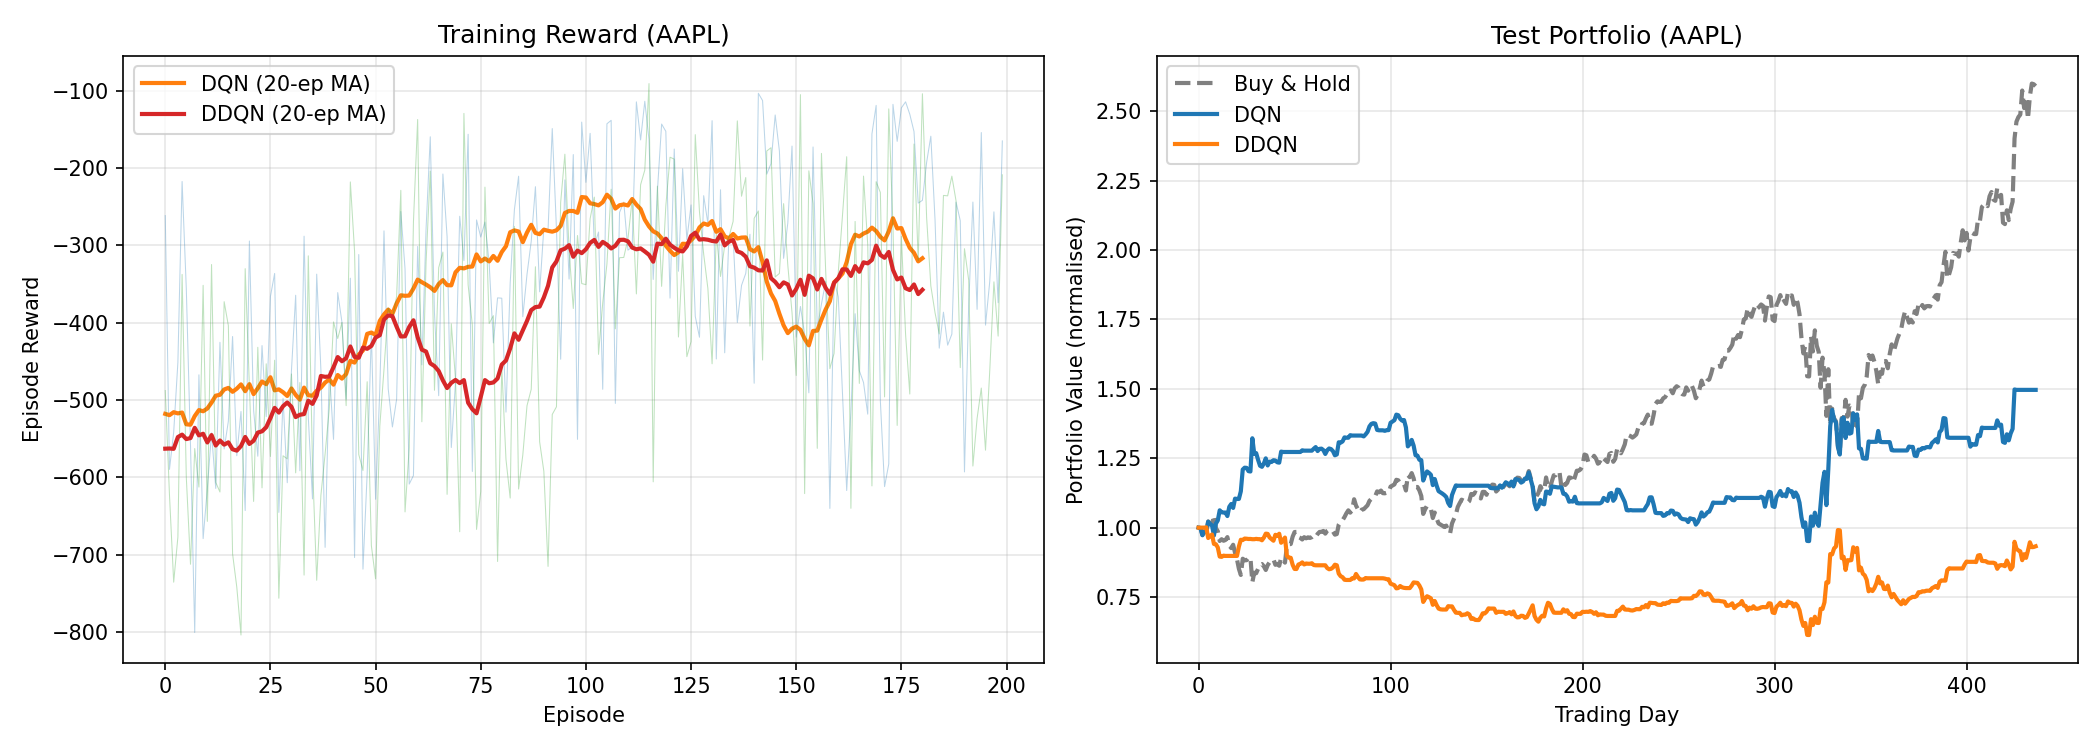
\includegraphics[width=0.95\textwidth]{results/results_AAPL.png}
  \caption{\textbf{Left:} Training reward per episode, shown as a 20-episode moving average. \textbf{Right:} Test portfolio-value trajectories for the RL agents and classical baselines on AAPL over 2018--2020.}
  \label{fig:training}
\end{figure*}

\begin{table*}[t]
\centering
\small
\setlength{\tabcolsep}{4pt}
\caption{Test performance on AAPL over the 436-day test split (2018--2020). All methods operate in the long-and-flat subset of the position space. Best value in each row is shown in bold.}
\label{tab:results}
\begin{tabular}{l cccc cccc}
\toprule
& \textbf{DQN} & \textbf{DDQN} & \textbf{A2C} & \textbf{PPO} & \textbf{B\&H} & \textbf{ARIMA} & \textbf{Momentum} & \textbf{RF} \\
\midrule
Cum.\ Return   & $+171.7\%$ & $+172.5\%$ & $+182.9\%$ & $\mathbf{+184.3\%}$ & $+159.3\%$ & $+121.1\%$ & $+167.0\%$ & $+81.1\%$ \\
Sharpe         & $+2.73$    & $+2.73$    & $+2.79$    & $\mathbf{+2.81}$    & $+1.65$    & $+1.67$    & $+2.62$    & $+1.25$ \\
Max Drawdown   & $\mathbf{-15.5\%}$ & $-15.9\%$ & $-17.1\%$ & $-16.7\%$ & $-31.4\%$ & $-18.8\%$ & $-17.5\%$ & $-26.8\%$ \\
\bottomrule
\end{tabular}
\end{table*}

A detailed episode walkthrough showing position decisions, cumulative reward, and trade markers is provided in Appendix~\ref{app:results} (Figure~\ref{fig:walkthrough}).

The test period spans 2018 to 2020 and therefore includes the COVID-19 crash of early 2020, so it is a fairly severe out-of-sample stress test. The original from-scratch agents underperformed the passive benchmark, but the final version in Table~\ref{tab:results} reverses that result. All four RL agents exceed buy-and-hold in cumulative return and Sharpe, and all four reduce maximum drawdown substantially.

The strongest RL result is PPO, with a cumulative return of $+184.3\%$, Sharpe of $2.81$ and max drawdown of $-16.7\%$. A2C is close behind at $+182.9\%$ return and Sharpe $2.79$, while DQN and DDQN both reach about $+172\%$ return and Sharpe above $2.72$. The main reason is not a mysterious deep-network advantage. It is the combination of a state feature that exposes the 20-day momentum signal, supervised warm-starting from that signal and a checkpointing choice that avoids overfitting the short validation window. The RL agents remain editable, trainable policies, but their first useful behaviour comes from a simple trend-following prior.

The classical baselines help interpret the result. Buy-and-hold captures the full AAPL uptrend and delivers a strong $+159.3\%$ return, but its drawdown is $-31.4\%$. Momentum-20 reaches $+167.0\%$ return, Sharpe $2.62$ and a much smaller $-17.5\%$ drawdown. ARIMA performs respectably at $+121.1\%$, while Random Forest improves relative to the earlier feature set but still trails the RL agents. This reinforces the central lesson: raw model capacity is less important than exposing and stabilising a useful trading signal.

Table~\ref{tab:policy} in Appendix~\ref{app:policy} shows that the learned policies are not simply buy-and-hold copies. DQN spends 74.1\% of the test split long and 25.9\% flat, with 19 trades. A2C spends 75.0\% long and 25.0\% flat, with 17 trades. The policies therefore participate in the secular uptrend while stepping out during some weak regimes, which explains the drawdown improvement relative to buy-and-hold.

Taken together, the experiment illustrates three lessons from first principles. First, naive RL trading can easily underperform a simple passive benchmark, so implementation correctness and baseline comparisons are essential. Second, a simple financial prior can dramatically improve RL performance: the momentum feature and warm-start are more important than merely increasing model capacity. Third, TDQN-style counterfactual replay is a natural fit for off-policy value agents because each market step can cheaply teach the Q-network about actions it did not take.

%====================================================================
\section{Challenges}
%====================================================================

An early version of the environment used normalised returns with standard deviation close to one instead of raw returns for rewards, which produced unrealistic values. We fixed this by keeping \texttt{raw\_return} as a separate column in the dataframe. Initial linear $\varepsilon$-decay exhausted exploration too quickly and we switched to an exponential schedule to give a smoother exploration to exploitation transition. The MSE loss was sensitive to large reward outliers and was replaced with a Huber smooth-$\ell_1$ loss together with reward clipping to the range $[-1,1]$. Hard target-network copies caused training instability and were replaced by soft Polyak updates with $\tau \approx 0.005$. The largest performance issue was more conceptual: the first agents were asked to discover a momentum-style policy without being given a clean momentum feature or prior. Adding \texttt{mom20}, warm-starting from the 20-day momentum rule and using TDQN-style counterfactual replay for DQN/DDQN solved this failure mode.

%====================================================================
\section{Future Work}
%====================================================================

Natural extensions of this project include continuous-action actor-critic methods such as SAC or TD3 for direct position sizing, multi-asset portfolio environments that trade several DJIA tickers jointly, recurrent LSTM architectures for explicit temporal dependencies, walk-forward validation across multiple market regimes, and reward formulations based directly on Sharpe or CVaR rather than raw log-returns.

%====================================================================
\section{Contributions}
%====================================================================

\noindent\textbf{Yufan.}
\begin{itemize}[leftmargin=*, itemsep=1pt, topsep=2pt]
  \item Initial from-scratch implementation of the entire codebase.
  \item Data pipeline with Kaggle \texttt{alincijov/trading} via \texttt{kagglehub} and 10-feature engineering (return, momentum, RSI, MACD, Bollinger, ATR, OBV, MA deviations, normalised volume).
  \item Gym-style \texttt{TradingEnv} with drawdown-penalised reward, transaction cost models, portfolio tracking and Sharpe / drawdown / trade-frequency evaluation.
  \item Initial DQN and DDQN agent with \texttt{QNetwork}, replay buffer, target network and training loop.
  \item Random Forest baseline (200 trees on the same feature set).
  \item Data pipeline and training figures, appendix material, and most of the report writing.
\end{itemize}

\vspace{2pt}
\noindent\textbf{Rutwik.}
\begin{itemize}[leftmargin=*, itemsep=1pt, topsep=2pt]
  \item Refinements to the agent and environment: position-delta action space, Huber loss, reward clipping and log-return reward formulation.
  \item Exponential $\varepsilon$-decay and soft Polyak target-network updates.
  \item Random-window training episodes and best-model checkpointing.
  \item Hyperparameter retuning (learning rate, batch size, buffer capacity).
  \item Classical baselines: buy-and-hold, ARIMA(1,0,0) walk-forward and 20-day momentum, integrated into the reporting and plotting flow.
  \item Performance-improvement pass with \texttt{mom20}, supervised momentum warm-starting, lower-destructive DQN exploration and TDQN-style counterfactual replay.
\end{itemize}

\vspace{2pt}
\noindent\textbf{Xin Fei.}
\begin{itemize}[leftmargin=*, itemsep=1pt, topsep=2pt]
  \item Implemented the additional actor-critic agents, including A2C and PPO, integrated them into the existing training and evaluation pipeline for comparison with DQN and DDQN.
  \item Analysed the actor-critic results against value-based RL agents and classical baselines.
\end{itemize}

%====================================================================
\begin{thebibliography}{99}

\bibitem{mnih2016a3c}
V.~Mnih, A.~P. Badia, M.~Mirza, et al.,
``Asynchronous methods for deep reinforcement learning,''
in \emph{ICML}, 2016.

\bibitem{schulman2017ppo}
J.~Schulman, F.~Wolski, P.~Dhariwal, A.~Radford, and O.~Klimov,
``Proximal policy optimization algorithms,''
\emph{arXiv preprint arXiv:1707.06347}, 2017.

\bibitem{sutton2018}
R.~S. Sutton and A.~G. Barto, \emph{Reinforcement Learning: An Introduction}, 2nd ed. MIT Press, 2018.

\bibitem{mnih2015}
V.~Mnih, K.~Kavukcuoglu, D.~Silver, et al., ``Human-level control through deep reinforcement learning,'' \emph{Nature}, vol.~518, no.~7540, pp.~529--533, 2015.

\bibitem{hasselt2016}
H.~van Hasselt, A.~Guez, and D.~Silver, ``Deep reinforcement learning with double Q-learning,'' in \emph{AAAI}, 2016, pp.~2094--2100.

\bibitem{lin1992}
L.-J. Lin, ``Self-improving reactive agents based on reinforcement learning, planning and teaching,'' \emph{Machine Learning}, vol.~8, no.~3--4, pp.~293--321, 1992.

\bibitem{polyak1992}
B.~T. Polyak and A.~B. Juditsky, ``Acceleration of stochastic approximation by averaging,'' \emph{SIAM Journal on Control and Optimization}, vol.~30, no.~4, pp.~838--855, 1992.

\bibitem{kingma2015}
D.~P. Kingma and J.~Ba, ``Adam: A method for stochastic optimization,'' in \emph{ICLR}, 2015.

\bibitem{brockman2016}
G.~Brockman, V.~Cheung, L.~Pettersson, et al., ``OpenAI Gym,'' \emph{arXiv preprint arXiv:1606.01540}, 2016.

\bibitem{paszke2019}
A.~Paszke, S.~Gross, F.~Massa, et al., ``PyTorch: An imperative style, high-performance deep learning library,'' in \emph{NeurIPS}, 2019, pp.~8024--8035.

\bibitem{moody2001}
J.~Moody and M.~Saffell, ``Learning to trade via direct reinforcement,'' \emph{IEEE Transactions on Neural Networks}, vol.~12, no.~4, pp.~875--889, 2001.

\bibitem{deng2016}
Y.~Deng, F.~Bao, Y.~Kong, Z.~Ren, and Q.~Dai, ``Deep direct reinforcement learning for financial signal representation and trading,'' \emph{IEEE Transactions on Neural Networks and Learning Systems}, vol.~28, no.~3, pp.~653--664, 2016.

\bibitem{jiang2017}
Z.~Jiang, D.~Xu, and J.~Liang, ``A deep reinforcement learning framework for the financial portfolio management problem,'' \emph{arXiv preprint arXiv:1706.10059}, 2017.

\bibitem{yang2020}
H.~Yang, X.-Y. Liu, S.~Zhong, and A.~Walid, ``Deep reinforcement learning for automated stock trading: An ensemble strategy,'' in \emph{ACM ICAIF}, 2020.

\bibitem{theate2021}
T.~Théate and D.~Ernst, ``An application of deep reinforcement learning to algorithmic trading,'' \emph{Expert Systems with Applications}, vol.~173, 2021.
\end{thebibliography}

%====================================================================
\appendix
\onecolumn

%====================================================================
\section{Data Pipeline Visualisations}
\label{app:data}
%====================================================================

\begin{figure}[H]
  \centering
  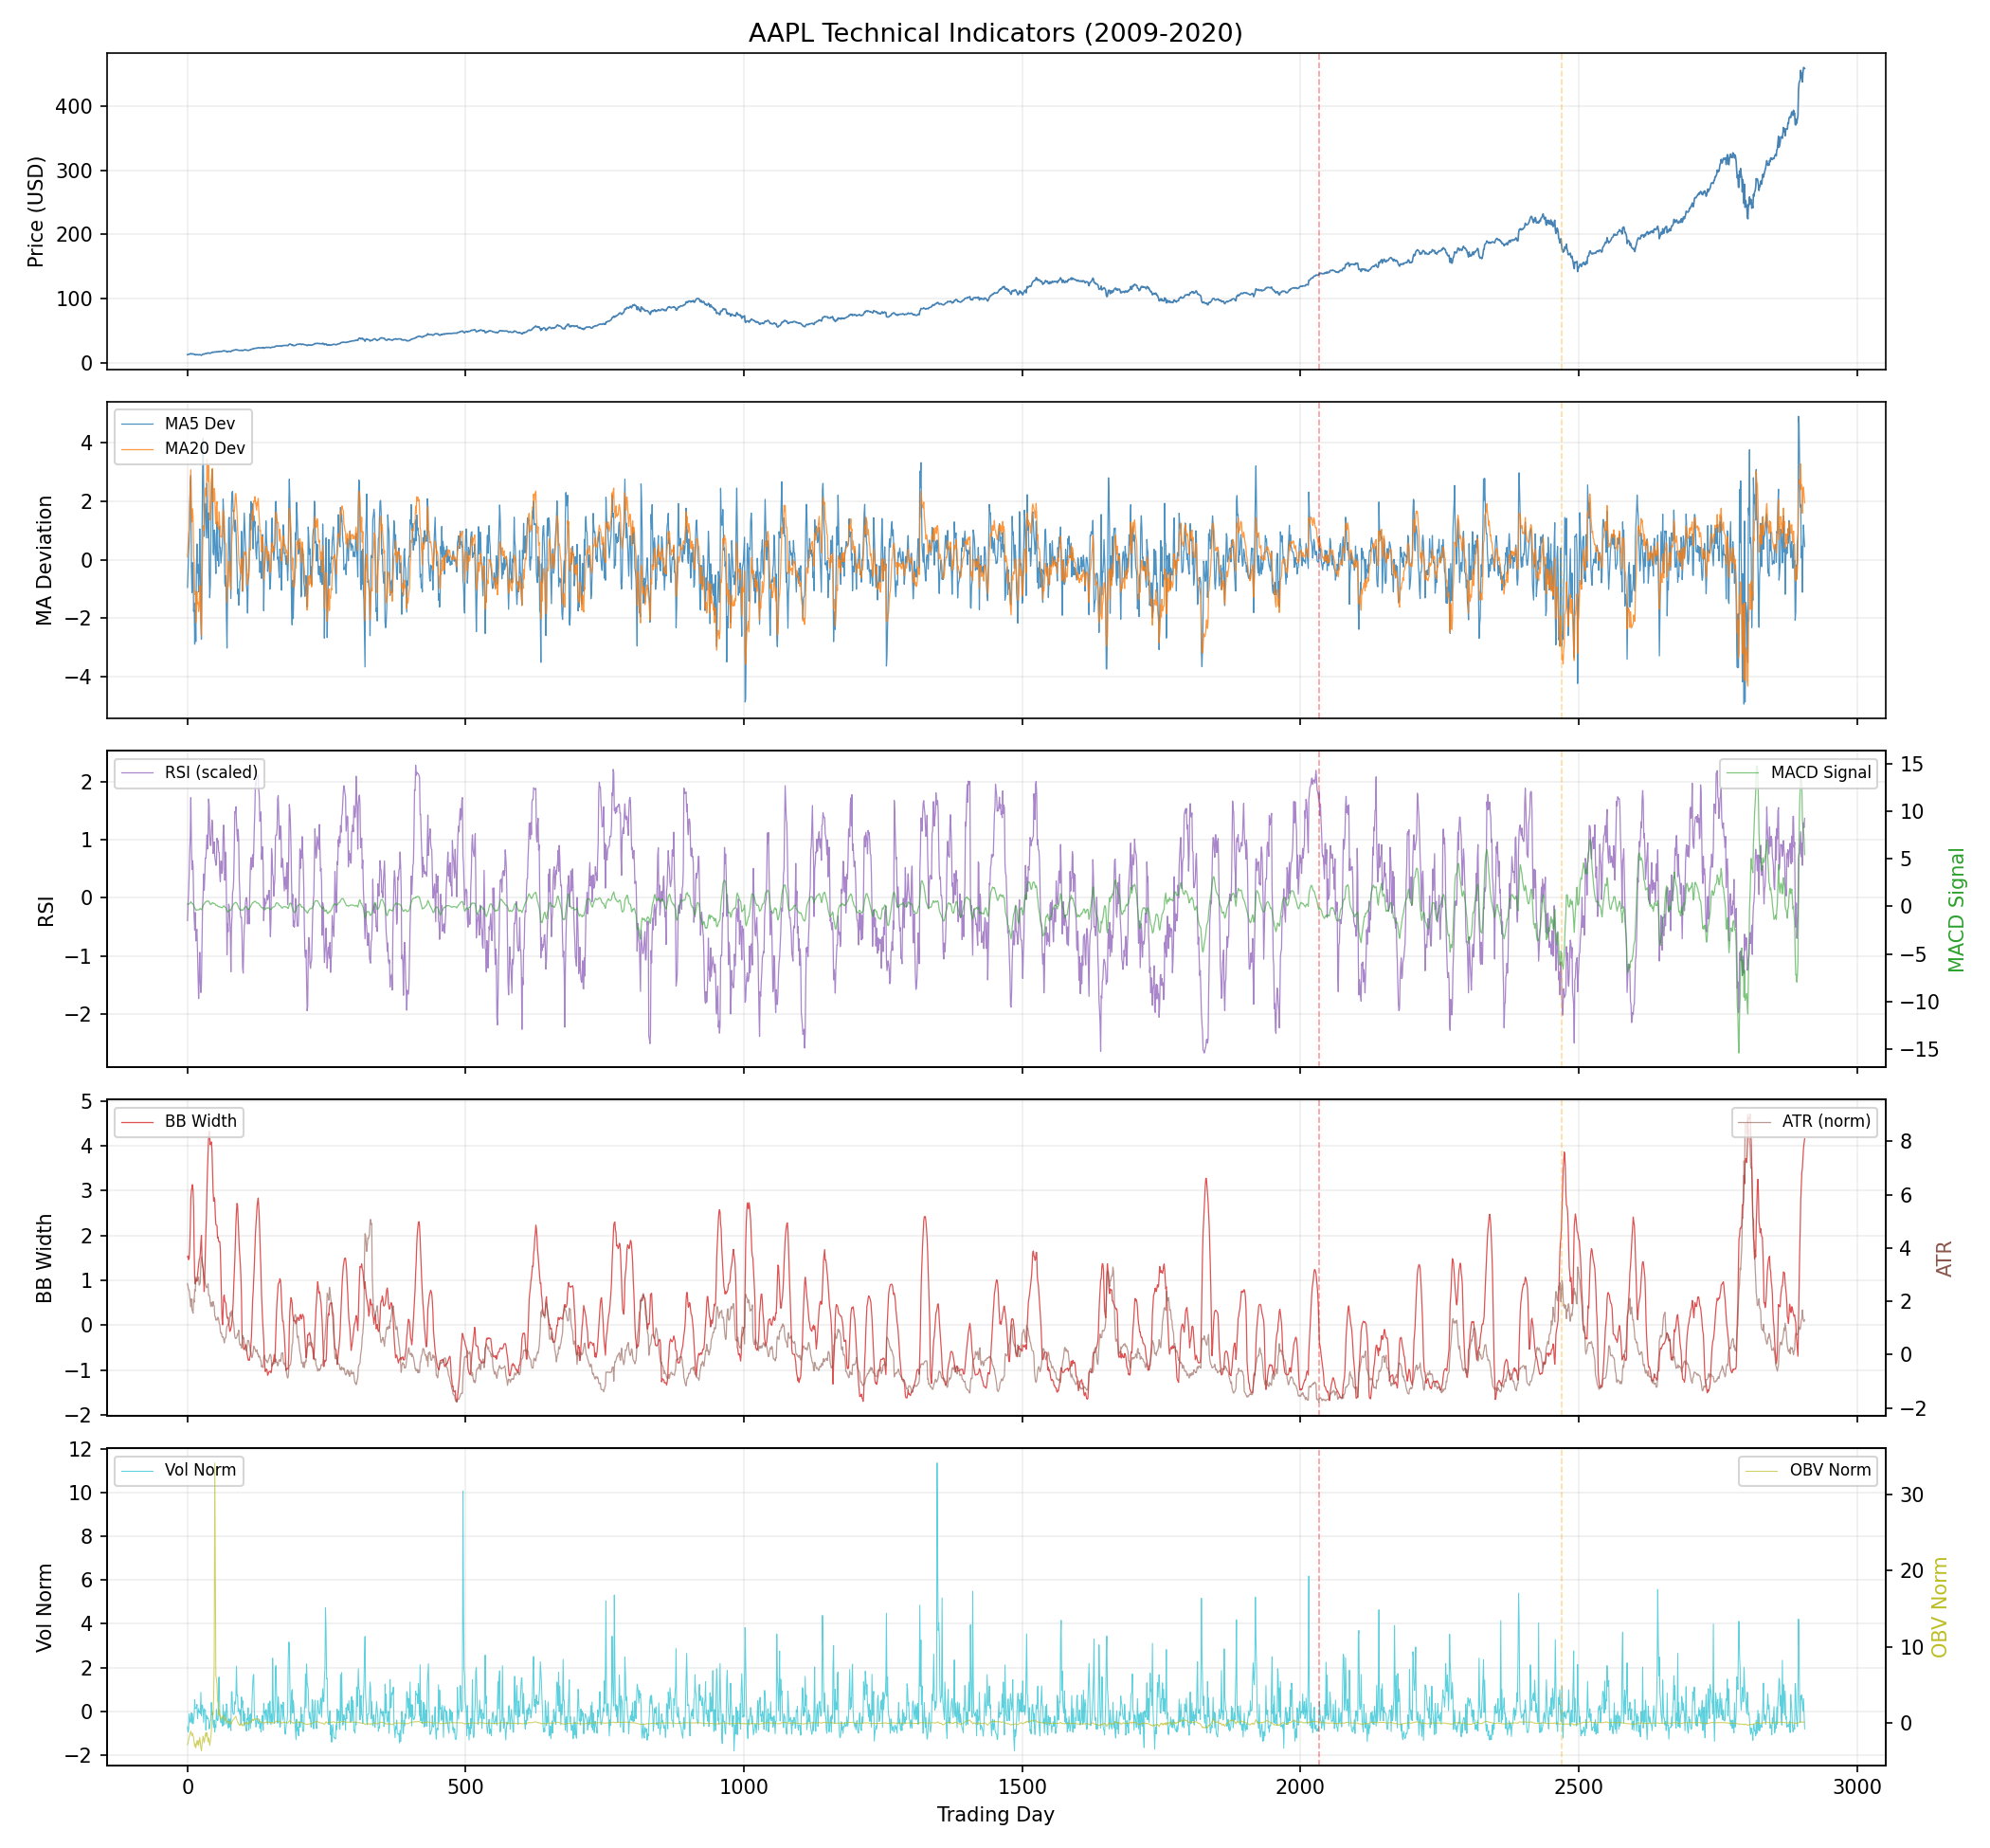
\includegraphics[width=0.95\textwidth]{results/technical_indicators.png}
  \caption{Technical indicator time series for AAPL (2009--2020). From top: close price, MA deviations, RSI \& MACD, Bollinger width \& ATR, volume \& OBV. Dashed lines mark train/val/test boundaries.}
  \label{fig:indicators}
\end{figure}

\begin{figure}[H]
  \centering
  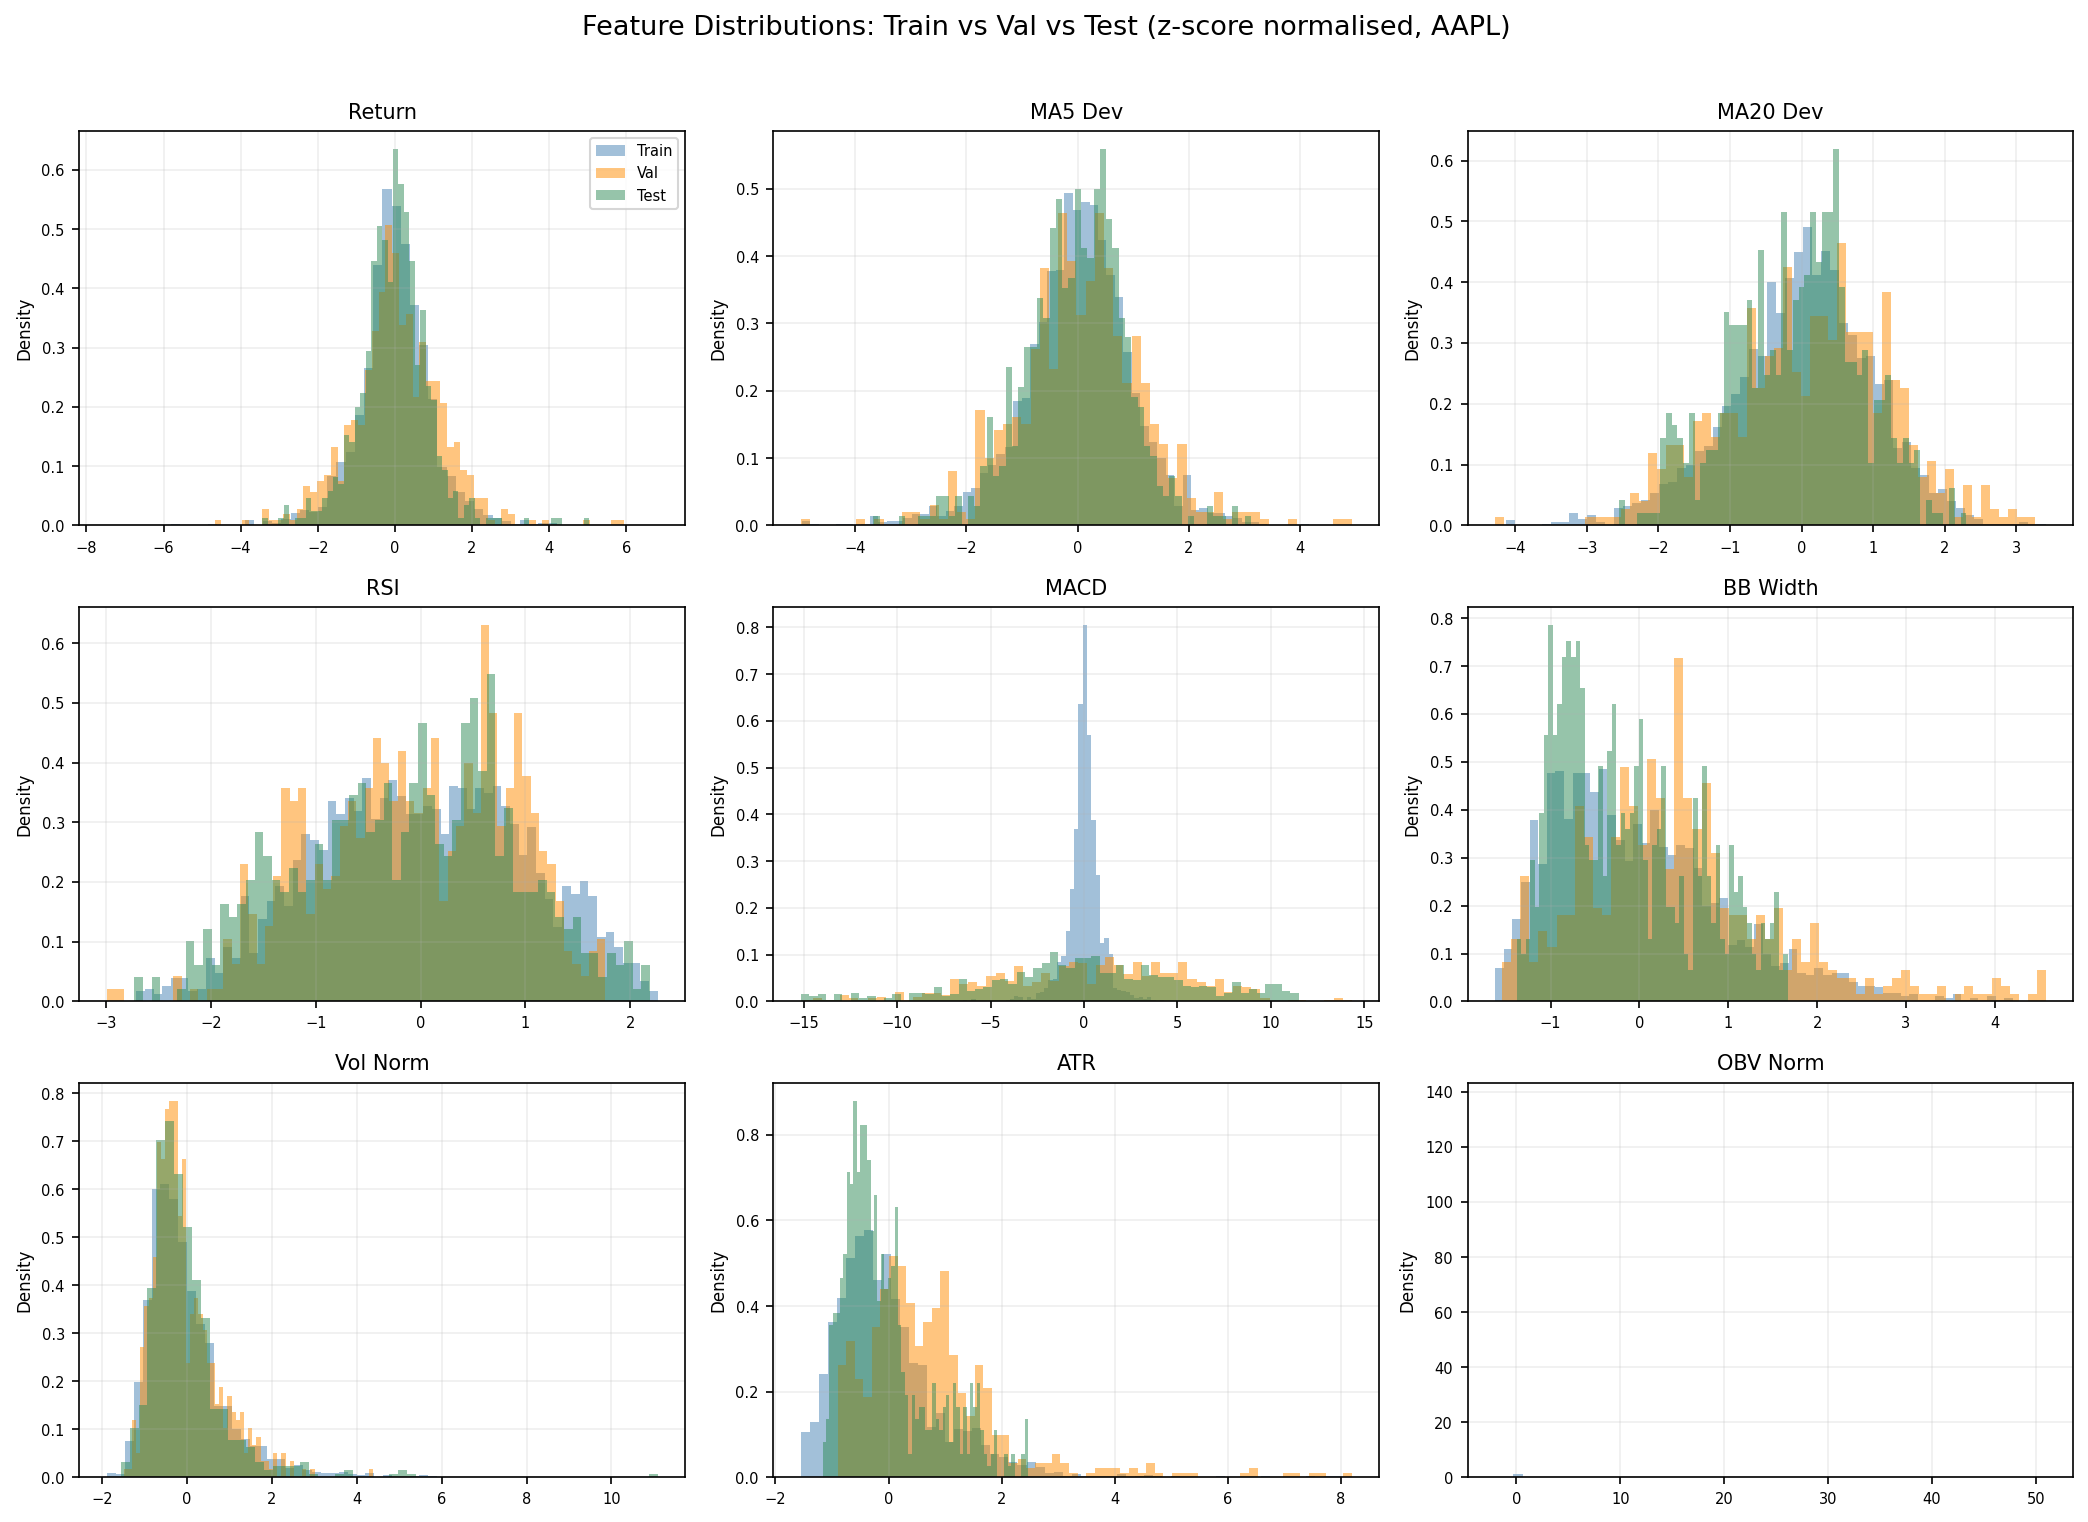
\includegraphics[width=0.95\textwidth]{results/feature_distributions.png}
  \caption{Feature distributions across train/val/test splits (z-score normalised using training-set statistics only). Overlapping distributions confirm consistent normalisation without look-ahead bias.}
  \label{fig:distributions}
\end{figure}

%====================================================================
\section{Policy Behaviour on the Test Split}
\label{app:policy}
%====================================================================

Table~\ref{tab:policy} reports position and trading statistics for the four RL agents and the four classical baselines, measured on the same 436-day AAPL test split (2018--2020) used for the headline metrics in Table~\ref{tab:results}. For each method we report the fraction of test steps spent long, flat or short, the total number of position changes over the split, and the trade rate expressed as a percentage of test days on which a position change occurred. All final experiments operate in the long-and-flat subset of the position space.

\begin{table}[H]
\centering
\small
\caption{Position and trading statistics on the AAPL test split. Fractions are percentages of the 436 test days. The trade rate is the number of position changes divided by the number of test days.}
\label{tab:policy}
\begin{tabular}{lcccrr}
\toprule
 & \textbf{\% Long} & \textbf{\% Flat} & \textbf{\% Short} & \textbf{Trades} & \textbf{Trade rate} \\
\midrule
DQN              & $74.1$ & $25.9$ & $0.0$ &  19 & $4.4\%$ \\
DDQN             & $74.5$ & $25.5$ & $0.0$ &  17 & $3.9\%$ \\
A2C              & $75.0$ & $25.0$ & $0.0$ &  17 & $3.9\%$ \\
PPO              & $74.8$ & $25.2$ & $0.0$ &  17 & $3.9\%$ \\
\midrule
Buy-and-Hold     & $100.0$ & $0.0$  & $0.0$ &   0 & $0.0\%$  \\
ARIMA(1,0,0)     & $68.8$  & $31.2$ & $0.0$ & 145 & $33.3\%$ \\
Momentum-20      & $76.1$  & $23.9$ & $0.0$ &  21 & $4.8\%$  \\
Random Forest    & $58.5$  & $41.5$ & $0.0$ & 175 & $40.1\%$ \\
\bottomrule
\end{tabular}
\end{table}

Three observations stand out. First, the best-performing RL agents and Momentum-20 all spend roughly three quarters of the test split long and one quarter flat. They therefore capture most of the secular AAPL uptrend while avoiding some weaker regimes. Second, the Random Forest classifier is still much more active than the RL agents, with 175 trades, so raw classifier capacity does not translate into stable high-level trading decisions. Third, the value-based and actor-critic policies converge to very similar position statistics after warm-starting, which explains why their headline performance is also close.

%====================================================================
\section{Episode Walkthrough}
\label{app:results}
%====================================================================

\begin{figure}[H]
  \centering
  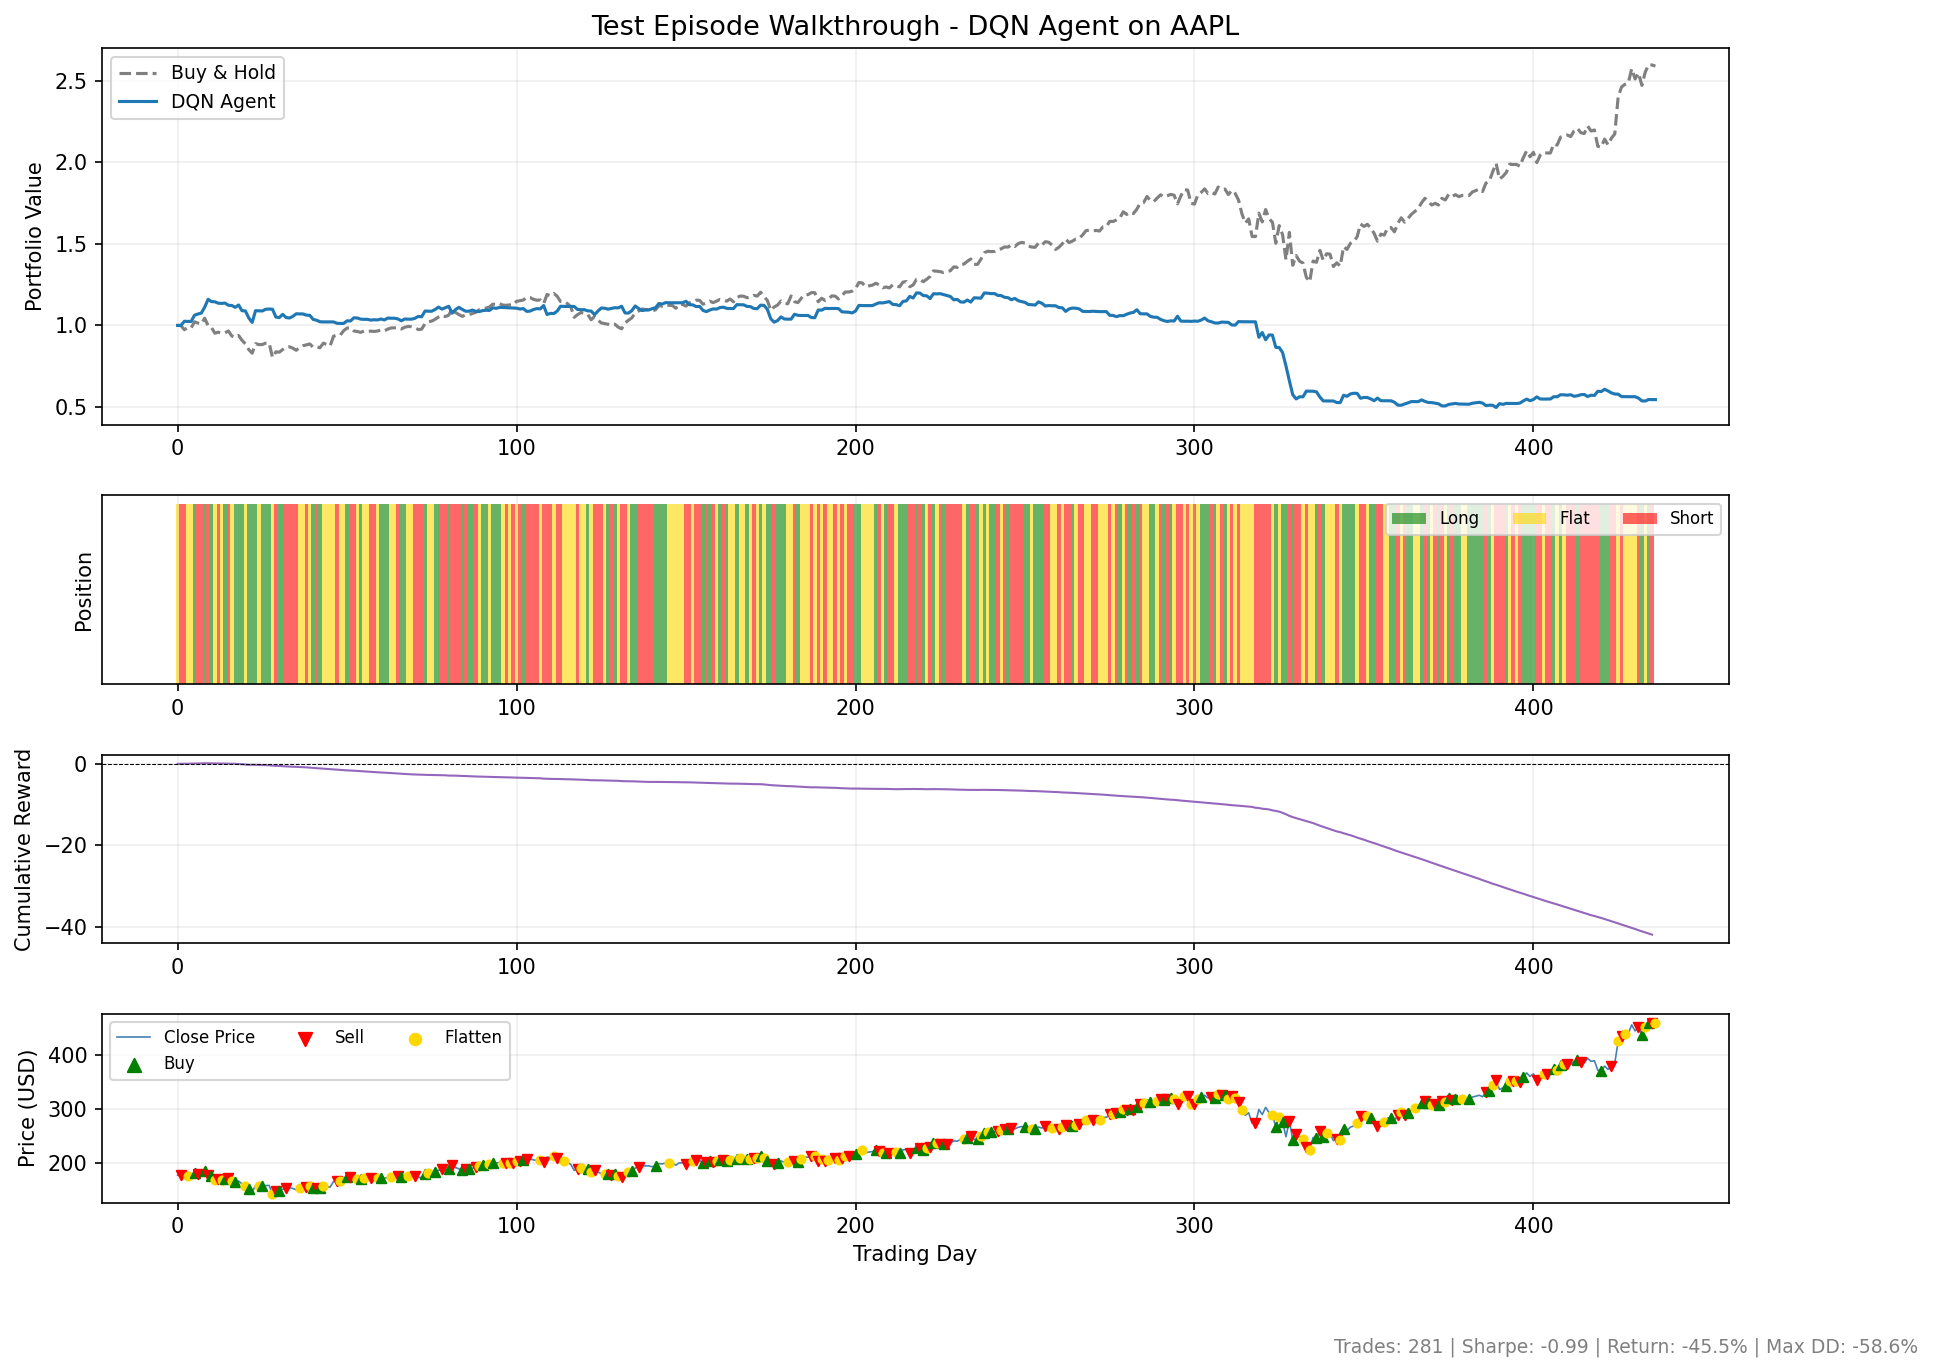
\includegraphics[width=0.95\textwidth]{results/episode_walkthrough.png}
  \caption{DQN test episode walkthrough on AAPL. Top: portfolio value vs buy-and-hold. Second: position colour bands (green=long, gold=flat). Third: cumulative reward. Bottom: buy/sell markers on close price.}
  \label{fig:walkthrough}
\end{figure}

\end{document}
